% answers.tex —— 1989 年·上海卷 · 参考答案与详细解析片段
% 由 tools/generate_projects.py 依来源总账自 1989/1989_数学真题_上海_试题.md + 1989/1989_数学真题_上海_解析正文.md + 1989/1989_数学真题_上海_答案要点.md 生成，勿手改（改源 MD 后重跑）


\begin{gktip}
固定源 PDF 印刷页 5-7—5-9 印有“上海数学试题解答”。下文将其推导规范化转录；第二大题固定源只给答案代号，所附简析为独立推导，不作为固定源原文或官方解析。
\end{gktip}

\begin{answer}
\gksolhead{1}{}

\textbf{题目}：

一、填空题

\Needspace{5\baselineskip}
（1） 若点 $P(1,a)$ 在曲线

\nopagebreak[4]
\[
x^2+2xy-5y=0
\]

上，则 $a=\underline{\hspace{4em}}$。

\Needspace{5\baselineskip}
（2） 计算

\nopagebreak[4]
\[
\frac{2\left(\cos\dfrac\pi3+i\sin\dfrac\pi3\right)^5}
{\sqrt2\left(\cos\dfrac\pi6+i\sin\dfrac\pi6\right)}
\]

（$i$ 为虚数单位），结果为 $\underline{\hspace{4em}}$。

\Needspace{5\baselineskip}
（3） 三角方程

\nopagebreak[4]
\[
\cos\left(\frac{x}{2}+\frac\pi3\right)=-\frac12
\]

的解集是 $\underline{\hspace{6em}}$。

（4） 侧棱长为 $3\text{ cm}$、底面边长为 $4\text{ cm}$ 的正四棱锥的体积为 $\underline{\hspace{4em}}\text{ cm}^3$。

（5） 函数 $y=x^{-2/3}$ 的递增区间是 $\underline{\hspace{4em}}$。

（6） 已知长方体 $ABCD-A'B'C'D'$ 中，棱 $AA'=5$，$AB=12$，如图。直线 $B'C'$ 和平面 $A'BCD'$ 的距离是 $\underline{\hspace{5em}}$。
\nopagebreak[4]
\begin{center}% 1989 年上海卷第一题第 6 小题：长方体 ABCD-A'B'C'D' 示意图；透视比例不代表题设尺寸
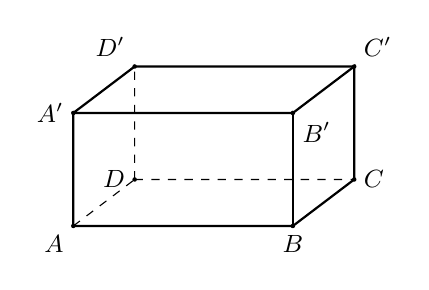
\begin{tikzpicture}[scale=0.82,>=stealth,font=\small]
  \coordinate (A) at (0,0);
  \coordinate (B) at (3.4,0);
  \coordinate (C) at (4.35,0.72);
  \coordinate (D) at (0.95,0.72);
  \coordinate (Ap) at (0,1.75);
  \coordinate (Bp) at (3.4,1.75);
  \coordinate (Cp) at (4.35,2.47);
  \coordinate (Dp) at (0.95,2.47);
  \draw[thick] (A)--(B)--(C)--(Cp)--(Bp)--(Ap)--cycle;
  \draw[thick] (Ap)--(Dp)--(Cp);
  \draw[thick] (A)--(Ap) (B)--(Bp);
  \draw[dashed] (A)--(D) (D)--(C) (D)--(Dp);
  \fill (A) circle (1pt) node[below left] {$A$};
  \fill (B) circle (1pt) node[below] {$B$};
  \fill (C) circle (1pt) node[right] {$C$};
  \fill (D) circle (1pt) node[left] {$D$};
  \fill (Ap) circle (1pt) node[left] {$A'$};
  \fill (Bp) circle (1pt) node[below right] {$B'$};
  \fill (Cp) circle (1pt) node[above right] {$C'$};
  \fill (Dp) circle (1pt) node[above left] {$D'$};
\end{tikzpicture}
\end{center}
\nopagebreak[4]
\Needspace{5\baselineskip}
（7） 方程

\nopagebreak[4]
\[
\log_2(x-3)=\log_4(5-x)
\]

的解是 $\underline{\hspace{4em}}$。

\Needspace{5\baselineskip}
（8） 已知 $\sin\alpha=\dfrac13$，$2\pi<\alpha<3\pi$，那么

\nopagebreak[4]
\[
\sin\frac\alpha2+\cos\frac\alpha2=
\]

 $\underline{\hspace{4em}}$。

\Needspace{5\baselineskip}
（9） 计算

\nopagebreak[4]
\[
\lim_{n\to\infty}\left(\frac1{n^2}+\frac4{n^2}+\frac7{n^2}+\cdots+\frac{3n-2}{n^2}\right)
\]

 $\underline{\hspace{4em}}$。

（10） 抛物线 $y=4x^2-4x$ 的准线方程是 $\underline{\hspace{4em}}$。

\Needspace{4\baselineskip}
\textbf{解析}

\gksubpart{（1）}

\Needspace{5\baselineskip}
将 $P(1,a)$ 代入曲线方程：

\nopagebreak[4]
\[
1+2a-5a=0\text{，}
\]

所以 $a=\dfrac13$。

\gksubpart{（2）}

\Needspace{5\baselineskip}
用复数的三角形式进行乘除：

\nopagebreak[4]
\[
\frac{2\operatorname{cis}^5(\pi/3)}{\sqrt2\operatorname{cis}(\pi/6)}
=\sqrt2\operatorname{cis}\left(\frac{5\pi}3-\frac\pi6\right)
=\sqrt2\operatorname{cis}\frac{3\pi}2
=-\sqrt2 i\text{。}
\]

\gksubpart{（3）}

\Needspace{5\baselineskip}
令 $\theta=\dfrac{x}{2}+\dfrac\pi3$。由 $\cos\theta=-\dfrac12$，有

\nopagebreak[4]
\[
\theta=\frac{2\pi}3+2k\pi\quad\text{\text{或}}\quad\theta=\frac{4\pi}3+2k\pi\text{，}\qquad k\in\mathbb Z\text{。}
\]

\Needspace{5\baselineskip}
因此

\nopagebreak[4]
\[
x=4k\pi+\frac{2\pi}3\quad\text{\text{或}}\quad x=4k\pi-2\pi\text{，}\qquad k\in\mathbb Z\text{。}
\]

\gksubpart{（4）}

\Needspace{5\baselineskip}
正四棱锥底面边长为 $4$，底面中心到顶点的距离为底面对角线的一半，即 $2\sqrt2$。由侧棱长为 $3$ 得高

\nopagebreak[4]
\[
h=\sqrt{3^2-(2\sqrt2)^2}=1\text{。}
\]

\Needspace{5\baselineskip}
所以体积为

\nopagebreak[4]
\[
V=\frac13\cdot4^2\cdot1=\frac{16}3\text{ cm}^3\text{。}
\]

\gksubpart{（5）}

\Needspace{5\baselineskip}
函数定义域为 $x\ne0$，且

\nopagebreak[4]
\[
y'=-\frac23x^{-5/3}\text{。}
\]

当 $x<0$ 时 $y'>0$，故递增区间为 $(-\infty,0)$。

\gksubpart{（6）}

\Needspace{5\baselineskip}
设 $AD=d$，以 $A$ 为原点，令 $AB$、$AD$、$AA'$ 分别沿 $x,y,z$ 轴，则

\nopagebreak[4]
\[
A'=(0,0,5),\quad B=(12,0,0),\quad D'=(0,d,5),\quad B'=(12,0,5),\quad C'=(12,d,5)\text{。}
\]

\Needspace{5\baselineskip}
平面 $A'BCD'$ 的方程由三个不共线点确定为 $5x+12z-60=0$。直线 $B'C'$ 平行于 $y$ 轴，故与该平面平行；取线上点 $B'(12,0,5)$，点到平面的距离为

\nopagebreak[4]
\[
\frac{|5\cdot12+12\cdot5-60|}{\sqrt{5^2+12^2}}=\frac{60}{13}\text{。}
\]

\gksubpart{（7）}

\Needspace{5\baselineskip}
定义域要求 $3<x<5$。将底数统一为 $2$：

\nopagebreak[4]
\[
\log_2(x-3)=\frac12\log_2(5-x)
\quad\Longrightarrow\quad
(x-3)^2=5-x\text{。}
\]

解得 $x=1$ 或 $x=4$，结合定义域得 $x=4$。

\gksubpart{（8）}

\nopagebreak[4]
\[
\left(\sin\frac\alpha2+\cos\frac\alpha2\right)^2
=1+\sin\alpha=\frac43\text{。}
\]

由 $\sin\alpha=\dfrac13$ 且 $2\pi<\alpha<3\pi$ 可知 $\alpha$ 位于 $(2\pi,\dfrac{5\pi}2)$，于是 $\dfrac\alpha2$ 位于第三象限，两项之和为负。因此答案为 $-\dfrac{2\sqrt3}3$。

\gksubpart{（9）}

\nopagebreak[4]
\[
\frac1{n^2}+\frac4{n^2}+\cdots+\frac{3n-2}{n^2}
=\frac1{n^2}\sum_{k=1}^n(3k-2)
=\frac{3n^2-n}{2n^2}\longrightarrow\frac32\text{。}
\]

\gksubpart{（10）}

\Needspace{5\baselineskip}
配方得

\nopagebreak[4]
\[
y=4\left(x-\frac12\right)^2-1\text{。}
\]

\Needspace{5\baselineskip}
抛物线顶点纵坐标为 $-1$，且 $4p=\dfrac14$，故准线为

\nopagebreak[4]
\[
y=-1-\frac1{16}=-\frac{17}{16}\text{。}
\]

\gkanswer{答案（1）：$\dfrac13$}

\gkanswer{答案（2）：$-\sqrt2 i$}

\gkanswer{答案（3）：$x=4k\pi+\dfrac{2\pi}3$ 或 $x=4k\pi-2\pi$，$k\in\mathbb Z$}

\gkanswer{答案（4）：$\dfrac{16}3\text{ cm}^3$}

\gkanswer{答案（5）：$(-\infty,0)$}

\gkanswer{答案（6）：$\dfrac{60}{13}$}

\gkanswer{答案（7）：$x=4$}

\gkanswer{答案（8）：$-\dfrac{2\sqrt3}3$}

\gkanswer{答案（9）：$\dfrac32$}

\gkanswer{答案（10）：$y=-\dfrac{17}{16}$}

\end{answer}
\begin{answer}
\gksolhead{2}{}

\textbf{题目}：

二、选择题

（1） 若 $\alpha$ 是第四象限的角，则 $\pi-\alpha$ 是\mbox{（　　）}

（A）第一象限的角　　（B）第二象限的角

（C）第三象限的角　　（D）第四象限的角

（2） 以点 $A(-5,4)$ 为圆心，且与 $x$ 轴相切的圆的标准方程是\mbox{（　　）}

（A）$(x+5)^2+(y-4)^2=16$

（B）$(x-5)^2+(y+4)^2=16$

（C）$(x+5)^2+(y-4)^2=25$

（D）$(x-5)^2+(y+4)^2=25$

（3） 若 $a<b<0$，则下列不等关系中不能成立的是\mbox{（　　）}

（A）$\dfrac1a>\dfrac1b$　　（B）$\dfrac1{a-b}>\dfrac1a$

（C）$|a|>|b|$　　（D）$a^2>b^2$

（4） 两排座位，第一排有 3 个座位，第二排有 5 个座位。若 8 名学生入座（每人一个座位），则不同坐法的种数是\mbox{（　　）}

（A）$C_8^5C_8^3$　　（B）$P_2^1C_8^5C_8^3$

（C）$P_8^5P_8^3$　　（D）$P_8^8$

（5） 设 $z_1,z_2$ 为复数，那么“$z_1^2+z_2^2=0$”是“$z_1,z_2$ 同时为零”的\mbox{（　　）}

（A）充分不必要条件　　（B）必要不充分条件

（C）充分必要条件　　（D）既不充分又不必要条件

（6） 下面四个函数中为奇函数的是\mbox{（　　）}

（A）$y=x^2\sin\left(x+\dfrac\pi2\right)$

（B）$y=x^2\cos\left(x+\dfrac\pi4\right)$

（C）$y=\cos(\operatorname{arc\,ctg}x)$

（D）$y=\operatorname{arc\,ctg}(\sin x)$

（7） 下列四个命题中的真命题是\mbox{（　　）}

（A）若直线 $l$ 与平面 $\alpha$ 内两条平行直线垂直，则 $l\perp\alpha$。

（B）若平面 $\alpha$ 内两条直线与平面 $\beta$ 内两条直线分别平行，则 $\alpha\parallel\beta$。

（C）若平面 $\alpha$ 与二面角 $\beta$-$MN$-$\gamma$ 的棱 $MN$ 交于点 $A$，与二面角的面 $\beta$、面 $\gamma$ 分别交于 $AB$、$AC$，则 $\angle BAC\le90^\circ$。

（D）以上三个命题都是假命题。

（8） 要得到函数 $y=\cos\left(2x-\dfrac\pi4\right)$ 的图象，只需将函数 $y=\sin 2x$ 的图象\mbox{（　　）}

（A）向左平移 $\dfrac\pi8$ 个单位　　（B）向右平移 $\dfrac\pi8$ 个单位

（C）向左平移 $\dfrac\pi4$ 个单位　　（D）向右平移 $\dfrac\pi4$ 个单位

（9） 设直角三角形 $\triangle ABC$ 的直角边 $BC=a$、$AC=b$，斜边 $AB=c$，且 $a<b$。分别以直线 $BC$、$AC$ 和 $AB$ 为轴将直角三角形绕轴旋转一周，所得三个旋转体的体积分别记为 $V_1,V_2,V_3$，那么 $V_1,V_2,V_3$ 间的大小关系是\mbox{（　　）}

（A）$V_3>V_1>V_2$　　（B）$V_1>V_2>V_3$

（C）$V_1>V_3>V_2$　　（D）$V_2>V_1>V_3$

（10） 下列参数方程（$t$ 是参数）中与方程 $y^2=x$ 表示同一曲线的是\mbox{（　　）}

（A）$\begin{cases}x=t,\\y=t^2;\end{cases}$
　（B）$\begin{cases}x=\sin^2t,\\y=\sin t;\end{cases}$

（C）$\begin{cases}x=t,\\y=\sqrt{|t|};\end{cases}$
　（D）$\begin{cases}x=\dfrac{1-\cos2t}{1+\cos2t},\\y=\operatorname{tg}t.\end{cases}$

\Needspace{4\baselineskip}
\textbf{解析}

据固定源答案表，选项依次为 $C,A,B,D,B,C,D,A,B,D$；以下为独立核验简析。

\gksubpart{（1）}

设 $\alpha=2\pi-\theta$，其中 $0<\theta<\dfrac\pi2$，则 $\pi-\alpha=\theta-\pi$，终边在第三象限，选 C。

\gksubpart{（2）}

圆心为 $(-5,4)$，与 $x$ 轴相切，半径为 $4$，故方程为 $(x+5)^2+(y-4)^2=16$，选 A。

\gksubpart{（3）}

\Needspace{5\baselineskip}
设 $u=-a$、$v=-b$，则 $u>v>0$。A、C、D 均成立；而

\nopagebreak[4]
\[
\frac1{a-b}=-\frac1{u-v}<-\frac1u=\frac1a\text{，}
\]

所以 B 所给不等式不可能成立，选 B。

\gksubpart{（4）}

8 名学生分别进入 8 个有区别的座位，坐法数为 $8!=P_8^8$，选 D。

\gksubpart{（5）}

若 $z_1=z_2=0$，则 $z_1^2+z_2^2=0$；反之不成立，例如 $z_1=1,z_2=i$。因此该等式是“二者同时为零”的必要不充分条件，选 B。

\gksubpart{（6）}

\Needspace{5\baselineskip}
在 $\operatorname{arc\,ctg}x\in(0,\pi)$ 的约定下，

\nopagebreak[4]
\[
\cos(\operatorname{arc\,ctg}x)=\frac{x}{\sqrt{1+x^2}}\text{，}
\]

是奇函数，选 C。

\gksubpart{（7）}

A 中只取平面内两条平行于 $x$ 轴的直线，再令 $l$ 平行于 $y$ 轴，便有 $l$ 垂直这两条直线却不垂直平面。B 中令 $\alpha:z=0$、$\beta:y=0$，两平面相交；在两平面内各取两条平行于其交线 $x$ 轴的直线，条件成立但两平面不平行。C 也不成立：取 $\beta:y=0$、$\gamma:y=x$、$\alpha:z=x+y$，令 $A=(0,0,0)$、$B=(-1,0,-1)$、$C=(1,1,2)$，则 $A$ 在两面交棱及平面 $\alpha$ 上，$B\in\alpha\cap\beta$、$C\in\alpha\cap\gamma$，且 $\overrightarrow{AB}\cdot\overrightarrow{AC}=-3<0$，故 $\angle BAC$ 为钝角。前三项皆假，D 真。

\gksubpart{（8）}

\nopagebreak[4]
\[
\cos\left(2x-\frac\pi4\right)=\sin\left(2x+\frac\pi4\right)
=\sin\left(2\left(x+\frac\pi8\right)\right)\text{，}
\]

故将 $y=\sin2x$ 向左平移 $\dfrac\pi8$，选 A。

\gksubpart{（9）}

分别绕 $BC$、$AC$ 旋转，所得圆锥体积为 $V_1=\dfrac13\pi b^2a$、$V_2=\dfrac13\pi a^2b$，所以 $V_1>V_2$。绕斜边旋转时圆锥底面半径为三角形对斜边的高 $ab/c$，故 $V_3=\dfrac13\pi (ab/c)^2c=\dfrac13\pi a^2b^2/c$；由 $b<c$ 得 $V_2>V_3$。因此 $V_1>V_2>V_3$，选 B。

\gksubpart{（10）}

选项 D 化为 $x=\tan^2t$、$y=\tan t$，参数取遍实数时正好得到 $y^2=x$，选 D。

\gkanswer{答案（1）：C}

\gkanswer{答案（2）：A}

\gkanswer{答案（3）：B}

\gkanswer{答案（4）：D}

\gkanswer{答案（5）：B}

\gkanswer{答案（6）：C}

\gkanswer{答案（7）：D}

\gkanswer{答案（8）：A}

\gkanswer{答案（9）：B}

\gkanswer{答案（10）：D}

\end{answer}
\begin{answer}
\gksolhead{3}{}

\textbf{题目}：

三、解答题

\Needspace{5\baselineskip}
（1） 求

\nopagebreak[4]
\[
\cos\left(2\operatorname{arc\,tg}\sqrt6+\frac\pi3\right)
\]

的值。

\Needspace{5\baselineskip}
（2） 求函数

\nopagebreak[4]
\[
y=\sqrt{2+\log_{1/2}x}+\sqrt{\operatorname{tg}x}
\]

的定义域。

（3） 在直角坐标系 $xOy$ 中，过点 $P(-3,4)$ 的直线 $l$ 与直线 $OP$ 的夹角为 $45^\circ$，求直线 $l$ 的方程。

（4） 在 $(1-x^2)^{20}$ 的展开式中，如果第 $4r$ 项和第 $r+2$ 项的二项式系数相等，

（1） 求 $r$ 的值；

（2） 写出展开式中的第 $4r$ 项和第 $r+2$ 项。

\Needspace{4\baselineskip}
\textbf{解析}

\gksubpart{（1）}

\Needspace{5\baselineskip}
令 $\theta=\operatorname{arc\,tg}\sqrt6$，则 $\tan\theta=\sqrt6$，从而

\nopagebreak[4]
\[
\cos2\theta=\frac{1-\tan^2\theta}{1+\tan^2\theta}=-\frac57\text{，}\qquad
\sin2\theta=\frac{2\tan\theta}{1+\tan^2\theta}=\frac{2\sqrt6}{7}\text{。}
\]

\Needspace{5\baselineskip}
所以

\nopagebreak[4]
\[
\cos\left(2\theta+\frac\pi3\right)
=\cos2\theta\cos\frac\pi3-\sin2\theta\sin\frac\pi3
=-\frac{5+6\sqrt2}{14}\text{。}
\]

\gksubpart{（2）}

\Needspace{5\baselineskip}
根式有意义要求

\nopagebreak[4]
\[
2+\log_{1/2}x\ge0\text{，}\qquad \operatorname{tg}x\ge0\text{。}
\]

\Needspace{5\baselineskip}
第一式给出 $0<x\le4$；第二式给出 $k\pi\le x<k\pi+\dfrac\pi2$，$k\in\mathbb Z$。取交集得

\nopagebreak[4]
\[
\left(0,\frac\pi2\right)\cup[\pi,4]\text{。}
\]

\gksubpart{（3）}

\Needspace{5\baselineskip}
直线 $OP$ 的斜率为 $-\dfrac43$。设直线 $l$ 的斜率为 $k$，由两直线夹角为 $45^\circ$，

\nopagebreak[4]
\[
\left|\frac{k+4/3}{1-4k/3}\right|=1\text{，}
\]

\Needspace{5\baselineskip}
解得 $k=-\dfrac17$ 或 $k=7$。结合 $P(-3,4)$，得到

\nopagebreak[4]
\[
x+7y-25=0\quad\text{\text{或}}\quad7x-y+25=0\text{。}
\]

\gksubpart{（4）}

\Needspace{5\baselineskip}
展开式第 $4r$ 项与第 $r+2$ 项的二项式系数分别为 $C_{20}^{4r-1}$、$C_{20}^{r+1}$。二项式系数相等当且仅当下标相同或下标之和为 $20$：

\nopagebreak[4]
\[
4r-1=r+1\quad\text{\text{或}}\quad(4r-1)+(r+1)=20\text{。}
\]

\Needspace{5\baselineskip}
前者得 $r=\dfrac23$，不符合项数条件；后者得 $r=4$。因此

\nopagebreak[4]
\[
T_{16}=C_{20}^{15}(-x^2)^{15}=-15504x^{30},\qquad
T_6=C_{20}^{5}(-x^2)^5=-15504x^{10}\text{。}
\]

\gkanswer{答案（1）：$-\dfrac{5+6\sqrt2}{14}$}

\gkanswer{答案（2）：$(0,\dfrac\pi2)\cup[\pi,4]$}

\gkanswer{答案（3）：$x+7y-25=0$ 或 $7x-y+25=0$}

\gkanswer{答案（4）：$r=4$；$T_{16}=-15504x^{30}$，$T_6=-15504x^{10}$}

\end{answer}
\begin{answer}
\gksolhead{4}{}

\textbf{题目}：

\Needspace{5\baselineskip}
四、如图，设点 $A\text{、}B$ 分别在二面角 $M$-$PQ$-$N$（平面角为锐角）的两个面 $N\text{、}M$ 上，直线 $AB$ 与面 $M\text{、}N$ 所成的角分别为 $\alpha\text{、}\beta$。过点 $A\text{、}B$ 分别作棱 $PQ$ 的垂线 $AE\text{、}BF$，垂足为 $E\text{、}F$。求证：

\nopagebreak[4]
\[
\frac{AE}{BF}=\frac{\sin\alpha}{\sin\beta}\text{。}
\]
\nopagebreak[4]
\begin{center}% 1989 年上海卷第四题：二面角及垂足示意；图形不表示精确角度或比例
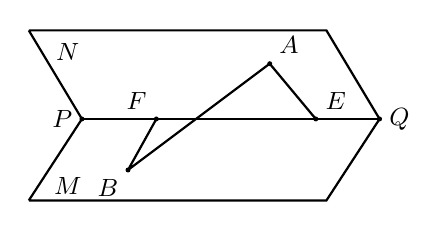
\begin{tikzpicture}[scale=0.9,>=stealth,font=\small]
  \coordinate (P) at (0,0);
  \coordinate (Q) at (4.2,0);
  \coordinate (N1) at (-0.75,1.25);
  \coordinate (N2) at (3.45,1.25);
  \coordinate (M1) at (-0.75,-1.15);
  \coordinate (M2) at (3.45,-1.15);
  \coordinate (A) at (2.65,0.78);
  \coordinate (B) at (0.65,-0.72);
  \coordinate (E) at (3.3,0);
  \coordinate (F) at (1.05,0);
  \draw[thick] (N1)--(N2)--(Q) (P)--(N1);
  \draw[thick] (M1)--(M2)--(Q) (P)--(M1);
  \draw[thick] (P)--(Q);
  \draw[thick] (A)--(B) (A)--(E) (B)--(F);
  \fill (P) circle (1pt) node[left] {$P$};
  \fill (Q) circle (1pt) node[right] {$Q$};
  \fill (A) circle (1pt) node[above right] {$A$};
  \fill (B) circle (1pt) node[below left] {$B$};
  \fill (E) circle (1pt) node[above right] {$E$};
  \fill (F) circle (1pt) node[above left] {$F$};
  \node at (-0.2,0.95) {$N$};
  \node at (-0.2,-0.95) {$M$};
\end{tikzpicture}
\end{center}
\nopagebreak[4]
\Needspace{4\baselineskip}
\textbf{解析}

\Needspace{5\baselineskip}
过 $A\text{、}B$ 分别作 $AC\perp M$、$BD\perp N$，垂足为 $C\text{、}D$，并连接 $CE\text{、}DF\text{、}BC\text{、}DA$。由直线与平面所成角的定义，

\nopagebreak[4]
\[
AC=AB\sin\alpha\text{，}\qquad BD=AB\sin\beta\text{。}
\]

\Needspace{5\baselineskip}
因为 $AE\perp PQ$、$BF\perp PQ$，由三垂线定理的逆定理有 $CE\perp PQ$、$DF\perp PQ$。于是 $\angle AEC$ 与 $\angle BFD$ 同为该二面角的平面角，故相等；直角三角形 $AEC$ 与 $BFD$ 相似，从而

\nopagebreak[4]
\[
\frac{AE}{BF}=\frac{AC}{BD}=\frac{AB\sin\alpha}{AB\sin\beta}
=\frac{\sin\alpha}{\sin\beta}\text{。}
\]
\nopagebreak[4]
\begin{center}% 1989 年上海卷第四题：二面角及垂足示意；图形不表示精确角度或比例
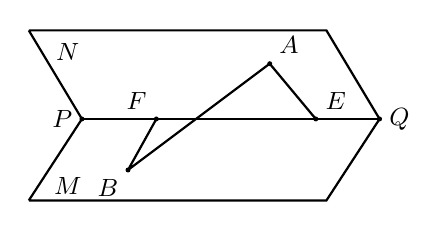
\begin{tikzpicture}[scale=0.9,>=stealth,font=\small]
  \coordinate (P) at (0,0);
  \coordinate (Q) at (4.2,0);
  \coordinate (N1) at (-0.75,1.25);
  \coordinate (N2) at (3.45,1.25);
  \coordinate (M1) at (-0.75,-1.15);
  \coordinate (M2) at (3.45,-1.15);
  \coordinate (A) at (2.65,0.78);
  \coordinate (B) at (0.65,-0.72);
  \coordinate (E) at (3.3,0);
  \coordinate (F) at (1.05,0);
  \draw[thick] (N1)--(N2)--(Q) (P)--(N1);
  \draw[thick] (M1)--(M2)--(Q) (P)--(M1);
  \draw[thick] (P)--(Q);
  \draw[thick] (A)--(B) (A)--(E) (B)--(F);
  \fill (P) circle (1pt) node[left] {$P$};
  \fill (Q) circle (1pt) node[right] {$Q$};
  \fill (A) circle (1pt) node[above right] {$A$};
  \fill (B) circle (1pt) node[below left] {$B$};
  \fill (E) circle (1pt) node[above right] {$E$};
  \fill (F) circle (1pt) node[above left] {$F$};
  \node at (-0.2,0.95) {$N$};
  \node at (-0.2,-0.95) {$M$};
\end{tikzpicture}
\end{center}
\nopagebreak[4]
\gkanswer{答案：见解析版}

\end{answer}
\begin{answer}
\gksolhead{5}{}

\textbf{题目}：

\Needspace{5\baselineskip}
五、设复数集合

\nopagebreak[4]
\[
M=\{z\mid |z-2+i|\le2,\ z\in\mathbb C\}\cap\{z\mid |z-2-i|=|z-4+i|,\ z\in\mathbb C\}
\]

（1） 试在复平面内作出表示集合 $M$ 的图形，并说出图形的名称；

（2） 求集合 $M$ 中元素 $z$ 的辐角主值的范围；

（3） 求集合 $M$ 中元素 $z$ 的模的范围。

\Needspace{4\baselineskip}
\textbf{解析}

\gksubpart{（1）}

\Needspace{5\baselineskip}
令 $z=x+iy$。集合的两个条件分别表示圆盘

\nopagebreak[4]
\[
(x-2)^2+(y+1)^2\le4
\]

\Needspace{5\baselineskip}
以及到点 $(2,1)$、$(4,-1)$ 等距的直线。由等距条件得

\nopagebreak[4]
\[
(x-2)^2+(y-1)^2=(x-4)^2+(y+1)^2\text{，}
\]

\Needspace{5\baselineskip}
即 $x-y=3$。该直线与圆周交于

\nopagebreak[4]
\[
A(2+\sqrt2,\sqrt2-1)\text{，}\qquad B(2-\sqrt2,-\sqrt2-1)\text{，}
\]

因此 $M$ 表示线段 $AB$。
\nopagebreak[4]
\begin{center}% 1989 年上海卷第五题解答图：圆盘与直线 x-y=3 的交集线段
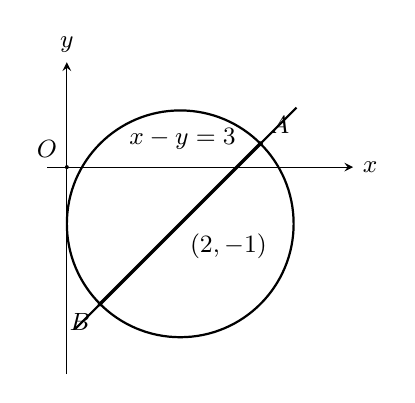
\begin{tikzpicture}[scale=0.72,>=stealth,font=\small]
  \draw[->] (-0.35,0)--(5.05,0) node[right] {$x$};
  \draw[->] (0,-3.65)--(0,1.85) node[above] {$y$};
  \draw[thick] (2,-1) circle[radius=2];
  \draw[thick] (0.15,-2.85)--(4.05,1.05);
  \draw[very thick] (2-1.41421356,-1-1.41421356)--(2+1.41421356,-1+1.41421356);
  \fill (0,0) circle (1pt) node[above left] {$O$};
  \fill (2+1.41421356,-1+1.41421356) circle (1.2pt)
    node[above right] {$A$};
  \fill (2-1.41421356,-1-1.41421356) circle (1.2pt)
    node[below left] {$B$};
  \node[below right] at (2,-1) {$(2,-1)$};
  \node[above left] at (3.15,0.15) {$x-y=3$};
\end{tikzpicture}
\end{center}
\nopagebreak[4]
\gksubpart{（2）}

\Needspace{5\baselineskip}
线段 $AB$ 与正实轴交于 $(3,0)$，两端点都在右半平面。由

\nopagebreak[4]
\[
\tan\arg A=\frac{\sqrt2-1}{2+\sqrt2}=\frac{3\sqrt2-4}{2},\qquad
\tan(2\pi-\arg B)=\frac{\sqrt2+1}{2-\sqrt2}=\frac{3\sqrt2+4}{2},
\]

\Needspace{5\baselineskip}
按 $[0,2\pi)$ 取辐角主值，得到

\nopagebreak[4]
\[
\arg z\in\left[2\pi-\operatorname{arctg}\frac{3\sqrt2+4}{2},2\pi\right)
\cup\left[0,\operatorname{arctg}\frac{3\sqrt2-4}{2}\right]\text{。}
\]

\gksubpart{（3）}

\Needspace{5\baselineskip}
线段上离原点最近的点是直线 $x-y=3$ 上的垂足 $P=(\dfrac32,-\dfrac32)$，故

\nopagebreak[4]
\[
|OP|=\frac{3\sqrt2}{2}\text{。}
\]

\Needspace{5\baselineskip}
端点模长满足 $|OA|^2=9+2\sqrt2$、$|OB|^2=9-2\sqrt2$，故模的范围为

\nopagebreak[4]
\[
\left[\frac{3\sqrt2}{2},\sqrt{9+2\sqrt2}\right]\text{。}
\]

\gkanswer{答案（1）：线段 $AB$，端点为 $A(2+\sqrt2,\sqrt2-1)$、$B(2-\sqrt2,-\sqrt2-1)$}

\gkanswer{答案（2）：$[2\pi-\operatorname{arctg}\dfrac{3\sqrt2+4}{2},2\pi)\cup[0,\operatorname{arctg}\dfrac{3\sqrt2-4}{2}]$}

\gkanswer{答案（3）：$[\dfrac{3\sqrt2}{2},\sqrt{9+2\sqrt2}]$}

\end{answer}
\begin{answer}
\gksolhead{6}{}

\textbf{题目}：

\Needspace{5\baselineskip}
六、已知等比数列 $\{a_n\}$ 的首项 $a_1>0$，公比 $q>-1$ 且 $q\ne0$。设数列 $\{b_n\}$ 的通项

\nopagebreak[4]
\[
b_n=a_{n+1}+a_{n+2}\qquad(n\in\mathbb N)
\]

数列 $\{a_n\}$、$\{b_n\}$ 的前 $n$ 项和分别记为 $A_n\text{、}B_n$。试比较 $A_n$ 与 $B_n$ 的大小。

\Needspace{4\baselineskip}
\textbf{解析}

\Needspace{5\baselineskip}
由 $a_n=a_1q^{n-1}$，

\nopagebreak[4]
\[
b_n=a_{n+1}+a_{n+2}=a_n(q+q^2)\text{，}\qquad B_n=(q+q^2)A_n\text{。}
\]

\Needspace{5\baselineskip}
因 $a_1>0$ 且 $q>-1$，几何级数前 $n$ 项和 $A_n>0$。于是

\nopagebreak[4]
\[
B_n-A_n=A_n(q^2+q-1)
=A_n\left(q+\frac{\sqrt5+1}{2}\right)
\left(q-\frac{\sqrt5-1}{2}\right)\text{。}
\]

在 $q>-1$ 范围内，第一因子为正。令 $\varphi=\dfrac{\sqrt5-1}{2}$，故当 $-1<q<\varphi$（并满足题设 $q\ne0$）时 $A_n>B_n$；当 $q=\varphi$ 时二者相等；当 $q>\varphi$ 时 $A_n<B_n$。

\gkanswer{答案：令 $\varphi=\dfrac{\sqrt5-1}{2}$；$-1<q<\varphi$ 且 $q\ne0$ 时 $A_n>B_n$，$q=\varphi$ 时 $A_n=B_n$，$q>\varphi$ 时 $A_n<B_n$。}

\end{answer}
\begin{answer}
\gksolhead{7}{}

\textbf{题目}：

\Needspace{5\baselineskip}
七、$F$ 是定点，$l$ 是定直线，点 $F$ 到直线 $l$ 的距离为 $p$（$p>0$）。点 $M$ 在直线 $l$ 上滑动，动点 $N$ 在 $MF$ 的延长线上，且满足条件

\nopagebreak[4]
\[
\frac{|FN|}{|MN|}=\frac1{|MF|}\text{。}
\]

（1） 求动点 $N$ 的轨迹；

（2） 求 $|MN|$ 的最小值。

\Needspace{4\baselineskip}
\textbf{解析}

\gksubpart{（1）}

\Needspace{5\baselineskip}
令 $K$ 为 $F$ 到 $l$ 的垂足，以 $F$ 为极点、$FK$ 的反向延长线为极轴，设 $N$ 的极坐标为 $(\rho,\theta)$。由图形关系，

\nopagebreak[4]
\[
|MF|=\frac{p}{\cos\theta},\qquad |FN|=\rho\text{，}\qquad |MN|=|MF|+|FN|\text{，}\qquad \rho>0,\ \cos\theta>0\text{。}
\]

\Needspace{5\baselineskip}
题设条件可改写为 $|FN|\,|MF|=|MN|$，即

\nopagebreak[4]
\[
\rho\frac p{\cos\theta}=\frac p{\cos\theta}+\rho\text{。}
\]

\Needspace{5\baselineskip}
因此轨迹的极坐标方程为

\nopagebreak[4]
\[
\rho=\frac1{1-\frac1p\cos\theta},\qquad 0<\cos\theta<p\text{。}
\]

其离心率为 $e=\dfrac1p$：$0<p<1$ 时为双曲线，$p=1$ 时为抛物线，$p>1$ 时为椭圆；在每种情形下均只取满足极坐标约束 $0<\cos\theta<p$ 的部分，其中 $l'$ 是过 $F$ 且垂直于 $l$ 的直线。
\nopagebreak[4]
\begin{center}% 1989 年上海卷第七题：题设几何关系及坐标示意；两图均不表示精确比例
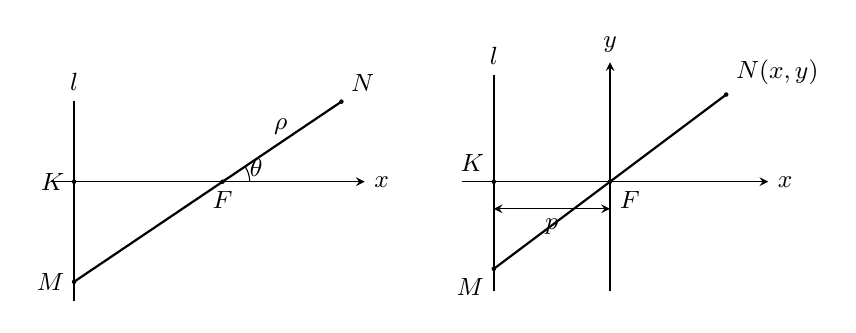
\begin{tikzpicture}[scale=0.82,>=stealth,font=\small]
  % Polar construction
  \begin{scope}
    \coordinate (K) at (0,0);
    \coordinate (F) at (2.3,0);
    \coordinate (M) at (0,-1.55);
    \coordinate (N) at (4.14,1.24);
    \draw[thick] (0,-1.85)--(0,1.25) node[above] {$l$};
    \draw[->] (-0.35,0)--(4.5,0) node[right] {$x$};
    \draw[thick] (M)--(N);
    \fill (K) circle (1pt) node[left] {$K$};
    \fill (F) circle (1pt) node[below] {$F$};
    \fill (M) circle (1pt) node[left] {$M$};
    \fill (N) circle (1pt) node[above right] {$N$};
    \draw (2.72,0) arc[start angle=0,end angle=33.98,radius=0.42];
    \node at (2.82,0.22) {$\theta$};
    \node at (3.2,0.85) {$\rho$};
  \end{scope}
  % Cartesian construction
  \begin{scope}[xshift=8.3cm]
    \coordinate (F) at (0,0);
    \coordinate (K) at (-1.8,0);
    \coordinate (M) at (-1.8,-1.35);
    \coordinate (N) at (1.8,1.35);
    \draw[thick] (-1.8,-1.7)--(-1.8,1.65) node[above] {$l$};
    \draw[->] (-2.3,0)--(2.45,0) node[right] {$x$};
    \draw[->] (0,-1.7)--(0,1.85) node[above] {$y$};
    \draw[thick] (M)--(N);
    \draw[<->] (-1.8,-0.42)--(0,-0.42) node[midway,below] {$p$};
    \fill (K) circle (1pt) node[above left] {$K$};
    \fill (F) circle (1pt) node[below right] {$F$};
    \fill (M) circle (1pt) node[below left] {$M$};
    \fill (N) circle (1pt) node[above right] {$N(x,y)$};
  \end{scope}
\end{tikzpicture}
\end{center}
\nopagebreak[4]
\gksubpart{（2）}

\Needspace{5\baselineskip}
又

\nopagebreak[4]
\[
|MN|=\frac p{\cos\theta}+\frac1{1-\frac1p\cos\theta}
=\frac{p^2}{\cos\theta\,(p-\cos\theta)}\text{。}
\]

令 $u=\cos\theta$，其中 $0<u\le1$ 且 $u<p$。若 $0<p\le2$，$u(p-u)$ 在允许的 $u=p/2$ 处取最大值 $p^2/4$（$p=2$ 时 $u=1$ 仍满足条件），从而 $|MN|$ 的最小值为 $4$。若 $p>2$，$u(p-u)$ 在 $0<u\le1$ 上递增，在 $u=1$ 处取最大值 $p-1$，故最小值为 $\dfrac{p^2}{p-1}$。

\gkanswer{答案（1）：$\rho=\dfrac1{1-\frac1p\cos\theta}$，其中 $0<\cos\theta<p$；$0<p<1$ 为双曲线部分，$p=1$ 为抛物线部分，$p>1$ 为椭圆部分}

\gkanswer{答案（2）：$4$（$0<p\le2$）；$\dfrac{p^2}{p-1}$（$p>2$）}

\end{answer}